\let\negmedspace\undefined
\let\negthickspace\undefined
\documentclass[journal,12pt,onecolumn]{IEEEtran}
\usepackage{cite}
\usepackage{amsmath,amssymb,amsfonts,amsthm}
\usepackage{algorithmic}
\usepackage{graphicx}
\graphicspath{{./figs/}}
\usepackage{textcomp}
\usepackage{xcolor}
\usepackage{txfonts}
\usepackage{listings}
\usepackage{enumitem}
\usepackage{mathtools}
\usepackage{gensymb}
\usepackage{comment}
\usepackage{caption}
\usepackage[breaklinks=true]{hyperref}
\usepackage{tkz-euclide} 
\usepackage{listings}
\usepackage{gvv}                                        
%\def\inputGnumericTable{}                                 
\usepackage[latin1]{inputenc}     
\usepackage{xparse}
\usepackage{color}                                            
\usepackage{array}
\usepackage{longtable}                                       
\usepackage{calc}                                             
\usepackage{multirow}
\usepackage{multicol}
\usepackage{hhline}                                           
\usepackage{ifthen}                                           
\usepackage{lscape}
\usepackage{tabularx}
\usepackage{array}
\usepackage{float}
\usepackage{parskip}
\newtheorem{theorem}{Theorem}[section]
\newtheorem{problem}{Problem}
\newtheorem{proposition}{Proposition}[section]
\newtheorem{lemma}{Lemma}[section]
\newtheorem{corollary}[theorem]{Corollary}
\newtheorem{example}{Example}[section]
\newtheorem{definition}[problem]{Definition}
\newcommand{\BEQA}{\begin{eqnarray}}
\newcommand{\EEQA}{\end{eqnarray}}
\newcommand{\define}{\stackrel{\triangle}{=}}
\theoremstyle{remark}
\newtheorem{rem}{Remark}

\begin{document}
\title{4.3.35}
\author{EE25BTECH11045 - P.Navya Priya}
\maketitle
\renewcommand{\thefigure}{\theenumi}
\renewcommand{\thetable}{\theenumi}
\textbf{Question:}

 Find the intercepts made by the plane $2\text{x} - 3\text{y} + 5\text{z} + 4 = 0$ on the co-ordinate axis 

\textbf{Solution:}
The above equation of plane can be written as
\begin{align*}
    \vec{n}^\top \vec{x}\,=\,\text{c}
\end{align*}
where 
\begin{align}
    \vec{n}=\myvec{2\\-3\\5}\\
    \text{c}=-4
\end{align}

Let the x-intercept of the given plane be of the form $\myvec{a\\0\\0}$. Substituting this in the above equation gives
\begin{align}
   \myvec{2\\-3\\5}^\top \myvec{a\\0\\0}\,&=\,-4\\
    \text{a}&=\,-2
\end{align}
\begin{align*}
    \therefore \,\text{The}\, x-\text{intercept \,is\,} \myvec{-2\\0\\0}
\end{align*}
Let the y-intercept of the given plane be of the form $\myvec{0\\b\\0}$. Substituting this in the above equation gives
\begin{align}
   \myvec{2\\-3\\5}^\top \myvec{0\\b\\0}\,&=\,-4\\
    \text{b}&=\,\frac{4}{3}
\end{align}
\begin{align*}
    \therefore \,\text{The}\, y-\text{intercept \,is\,} \myvec{0\\\frac{4}{3}\\0}
\end{align*}
    Let the z-intercept of the given plane be of the form $\myvec{0\\0\\c}$. Substituting this in the above equation gives
\begin{align}
   \myvec{2\\-3\\5}^\top \myvec{0\\0\\c}\,&=\,-4\\
    \text{c}&=\,\frac{-4}{5}
\end{align}
\begin{align*}
    \therefore \,\text{The}\, z-\text{intercept \,is\,} \myvec{0\\0\\\frac{-4}{5}}
\end{align*}

From the graph, theoretical solution matches with the computational solution.

\begin{figure}[H]
\centering
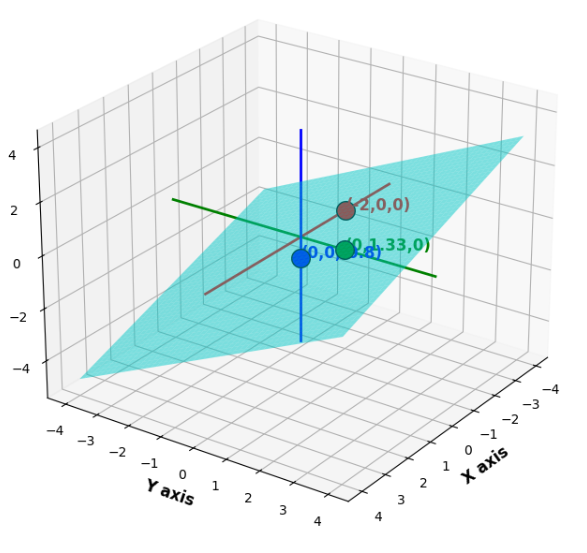
\includegraphics[width=0.7\columnwidth]{figs/graph.png}
\caption*{plane $2\text{x} - 3\text{y} + 5\text{z} + 4 = 0$ with intercepts}
\label{fig:graph.png}
\end{figure}
\end{document}